\documentclass[conference]{IEEEtran}
\IEEEoverridecommandlockouts
% The preceding line is only needed to identify funding in the first footnote. If that is unneeded, please comment it out.
\usepackage[nolist]{acronym}
%\usepackage{cite}
\usepackage{amsmath,amssymb,amsfonts}
\usepackage{algorithmic}
\usepackage{graphicx}
\usepackage{textcomp}
\usepackage{xcolor}
\usepackage{hyperref}
\usepackage{cleveref}
\usepackage{placeins}
\usepackage{blindtext}
\usepackage{multirow}
\usepackage{flushend} % comment out if too buggy
\usepackage[style=ieee]{biblatex}
\usepackage[inline]{enumitem}

\bibliography{./references.bib}
\bibliography{./references2.bib}
\thispagestyle{plain}
\pagestyle{plain}
% acronyms \ac{} for normal, will be full length for first mention. \acp{} for 
% plural (IoT => IoTs), \acf{} for full length
\begin{acronym}
\acro{iot}[IoT]{Internet of Things}
\end{acronym}
\begin{acronym}
\acro{faas}[FaaS]{Function-as-a-Service}
\end{acronym}
\begin{acronym}
\acro{rest}[REST]{Representational state transfer}
\end{acronym}
\begin{acronym}
\acro{paas}[PaaS]{Platform as a Service}
\end{acronym}
\begin{acronym}
\acro{gcp}[GCP]{Google Cloud Platform}
\end{acronym}
\begin{acronym}
\acro{cos}[COS]{Cloud Operating System}
\end{acronym}
\begin{acronym}
\acro{rtt}[RTT]{Round Trip Time}
\end{acronym}
\begin{acronym}
\acro{json}[JSON]{JavaScript Object Notation}
\end{acronym}

\def\BibTeX{{\rm B\kern-.05em{\sc i\kern-.025em b}\kern-.08em
    T\kern-.1667em\lower.7ex\hbox{E}\kern-.125emX}}

\begin{document}

\title{Syncmesh: Distributed Storage for \\Function As A Service\\
{\footnotesize Report for Distributed Systems Project 2021}
}

\author{\IEEEauthorblockN{Daniel Habenicht}
\IEEEauthorblockA{\textit{Student} \\
\textit{Technical University Berlin}\\
Berlin, Germany}
\and
\IEEEauthorblockN{Denis Koljada}
\IEEEauthorblockA{\textit{Student} \\
\textit{Technical University Berlin}\\
Berlin, Germany}
\and
\IEEEauthorblockN{Kevin Kreutz}
\IEEEauthorblockA{\textit{Student} \\
\textit{Technical University Berlin}\\
Berlin, Germany}
}

\maketitle

\begin{abstract}
In the current landscape of ongoing decentralization and distribution of data as well as computing itself, the coordination and synchronization of these aspects have become a fundamental question in distributed systems research. Specifically, in a localized environment with several data sources, the problem of querying and managing this data in a coordinated manner arises. To tackle this, we propose a custom solution that encompasses a unified system to manage and aggregate data in a scalable and stateless manner. We also evaluate and compare our approach to other established centralized and decentralized solutions, with the result of comparable performance regarding their request \acl{rtt} and outperforming the other solutions with regard to Total Traffic Flow. Our results suggest that the proposed solution is sufficient in specific, localized situations to mitigate the latency trade-off, with data distributed over multiple instances, while pertaining to the paradigms of a stateless, on-demand aggregation and query system.
\end{abstract}

% Find out what they want as structure. 
%- Publish paper on github

\section{Introduction}\label{Chap:Introduction}

With the recent increase in computational power and prevalence of mobile as well as smart devices, distributed networks have been growing in importance in the past years. More specifically, in the context of the \ac{iot}, aspects of scalability, local processing, and storage of data are of relevance. To tackle this trend, several solutions exist. One of the more prominent approaches is a centralized \ac{iot} cloud that provides the necessary infrastructure for the underlying network. However, different methods exist, such as distributed cloud infrastructures or even finer-grained, localized architectures that manage user requests directly to reduce latency and enable a more privacy-focused environment. With cloud solutions, the approach of \ac{faas} has been gaining in popularity. Various platforms, such as AWS Lambda, Google Cloud Functions, OpenFaas, or tinyFaas, provide on-demand computing as an alternative to full-fledged \ac{paas} options.

For \ac{iot} services that have high data velocity and volume, such a concept is of interest, as functions are stateless and horizontally scalable, consequently capable of fast consecutive queries and data handling. Currently, however, the main focus of \ac{faas} and serverless infrastructure normally lies within the coordination and management of small processes and operations, thus decoupling the server maintenance and management technicalities from the actual logic. This comes with the property and in some instances disadvantage, of data and state being managed separately from the function instances. In a distributed, highly localized context like \ac{iot} the challenge arises of coordinating these local states and communicating data between nodes. Several problems need to be addressed, namely how to design a data management system that both functions in a highly decentralized environment, but also carries the traditional principles of stateless and scalable operations.

In general, various solutions already exist for enabling distributed storage across a number of nodes, however none of them currently make use of certain advantages that exist within the implementation of management handled by \ac{faas}. Thus, the question regarding the implementation and feasibility of implementing such a distributed data storage system using \ac{faas} as a base mechanism, with a focus on \ac{iot} applications arises. As of now, no solution exists that directly combines the properties of distributed storage with the inherent advantages and effects of \ac{faas}, namely dynamic scalability, decreased latency in local scenarios, and reduced operation costs in contrast to more expansive systems, into a unified, standalone system. To address this gap, in this paper we propose a solution called \emph{Syncmesh} - a distributed data storage system that utilizes known \ac{faas} architecture and mechanisms.
With Syncmesh, we present a concept that enables a decentralized architecture of \ac{faas} instances within an \ac{iot} context. The instances can communicate with each other to propagate data queries and perform requests in a distributed, fully decentralized manner.

In the following chapters, we will outline the current research landscape regarding both state of the art distributed storage systems, as well as research concerning \ac{faas} in edge and fog environments. After outlining our approach in \Cref{Chap:Approach}, we describe the implementation of the proposed prototype and major functionality in \Cref{Chap:Prototype}, then evaluate the solution in \Cref{Chap:Eva} and benchmark it against different scenarios. Finally, \Cref{Chap:Conclusion} provides an overview of our findings and a short outlook addressing limitations and future research.

\section{Related Work}\label{Chap:RelatedWork}
\subsection{Distributed Storage}\label{Sec:Rel_Distributed}
In the last few decades, the amount of data produced, used and processed has been steadily increasing. With this increase, the demand for efficient data storage systems grows, and the requirements are constantly changing. 
Because of the requirement of fault tolerance in the form of reliability and availability, distributed database systems have proven themselves in recent years. Many companies have developed their own systems to tackle their own demands: Google with the Google File System (GFS) on which Apache Hadoop\footnote{\url{https://hadoop.apache.org/}} is based, Facebook with Cassandra\footnote{\url{https://cassandra.apache.org/}} and Amazon with Dynamo\footnote{\url{https://aws.amazon.com/de/dynamodb/}}.  Each of the currently available proposals and solutions comes with its specific advantages and trade-offs. More related to our examined scenarios, research exists evaluating the performance of some of the aforementioned systems in \ac{iot} and edge contexts \cite{performanceinfrastructure}.

The Google File System (GFS) \cite{googlefilesystem} was specifically developed to handle the huge amount of data produced by Google's services. GFS enables easy horizontal scaling using cheap hardware to tackle the fault tolerance requirements. Later on, the MapReduce paradigm was introduced which served as an important basis for further work in distributed data processing such as in HDFS, the Hadoop Distributed File System\footnote{\url{https://hadoop.apache.org/docs/r1.2.1/hdfs_design.html}}. These systems were some of the first to introduce the idea of efficiently splitting data up into chunks and then storing these chunks across multiple nodes.

Within the context of localized data storage and management, there exist various solutions regarding \ac{iot} and its specific needs. By definition, \ac{iot} as a highly distributed environment, already requires in a sense distributed storage systems, because sensors and \ac{iot} devices that are interconnected must often share data for communication purposes. While traditionally this is done using a centralized instance, it comes with various disadvantages. One system which was recently designed with the specific purpose of usage as a data management system for the \ac{iot} and to tackle issues arising from centralized approaches, is Nebulastream \cite{zeuch2020nebulastream}. The authors outline a data processing system that works in a distributed manner. The solution is evaluated with regard to specific \ac{iot} challenges and scenarios. 

Mayer et al. \cite{fogstore} also address data management problems within decentralized fog networks and introduce an own solution called "FogStore", which is a context-aware distributed data storage system. In addition to state management, the paper outlines specific replica placement strategies and a generalized API for querying and manipulating data. A network and data manipulation latency evaluation is also performed.

\subsection{Function As A Service}\label{Sec:Rel_Faas}
In addition to considering related work regarding distributed storage systems, it is relevant to look at research concerning \ac{faas} within the context of \ac{iot} and fog environments. This is of importance, as current research within the area of distributed storage mostly focuses on stateful systems, while stateless applications and the properties of \ac{faas} are mostly touched upon within other research areas. Especially for Edge Computing, there have recently been multiple commercial providers which enable a function-based approach, however we are interested in more research-oriented work.

As \ac{faas} platforms provide serverless on-demand and event-driven computing resources, this results in more flexibility and higher scalability \cite{Fox2017StatusResearch}. Consequently, for this paper, we are interested in the role \ac{faas} systems can play in the \ac{iot}, especially in edge environments and the resulting challenges in storage and orchestration \cite{Rani2021StorageReview}. As with distributed storage, \ac{faas} platforms have been examined regarding their performance, with proposals of generalized benchmarking systems to measure network latency and other metrics for \ac{iot} and edge environments in general \cite{GrambowBeFaaS:Platforms}.

With Fog Function, Cheng et al. \cite{fogfunction} explore \ac{faas} as a serverless programming model within the context of \ac{iot}, which uses event-listeners to discover and orchestrate devices and resources in \ac{iot} environments. The aim of the authors was to use the advantages of FaaS, namely efficiency and flexibility in \ac{iot} systems.
In addition to outlining several use cases and performing a performance evaluation, Fog function was applied to FogFlow, which is a framework for Fog computing with the goal of providing a programming model that enables programmers to develop \ac{iot} systems more easily \cite{Cheng2018FogFlow:Cities}.

Using \ac{faas} in combination with distributed environments has also been explored \cite{Barcelona-Pons2019OnArchitectures}, with a proposed system to distribute workloads across multiple nodes. Several common machine learning algorithm use cases were evaluated, such as clustering operations and logistic regression. The work introduces an additional layer in form of a data store that handles aspects regarding consistency and state management. In general, it is shown that \ac{faas} does work in a consistent manner with regard to state mutation and coordination, using an own approach to the specific problems discussed in the work.

\section{Approach}\label{Chap:Approach}
This chapter addresses the general problem requirements and outlines our proposed solution. Additionally, the used technologies and frameworks are specified.

\subsection{Architecture}\label{Sec:Architecture}
With \ac{iot} and its inherent properties, more specifically in the context of edge computing being the focus of this work, the question arises what properties our proposed system should encompass. The most important factors are the system of communication between nodes. From this, we extract the requirement of a defined and unified communication model for each node. Additionally, the question of data replication and transport between nodes is of relevance. For this, a predefined and consistent model of transporting, replicating and synchronizing data arises as a requirement.
In our specific use case, the problem consists of decentralized weather measurement nodes that record metrics such as temperature, pressure or humidity. The dataset was taken from an \ac{iot} network, measuring the air quality in the city of Sofia in Bulgaria\footnote{\url{https://airsofia.info/}}. An excerpt of the dataset is depicted in \autoref{tbl:csvHeaders}.

\begin{table}[!h]
\caption{Excerpt of the Dataset}
\label{tbl:csvHeaders}
\centering
\resizebox{\columnwidth}{!}{%
    \begin{tabular}{|c|c|c|c|c|c|c|c|}
    \hline
    sensor\_id & location & latitude & longitude & timestamp & pressure & temperature & humidity \\ \hline
    1764 & 879 & 42.622 & 23.366 & 2017-07-01T00:02:09 & 93920.2 & 24.65 & 47.32 \\ \hline
    1764 & 879 & 42.622 & 23.366 & 2017-07-01T00:04:35 & 93919.02 & 24.48 & 47.63 \\ \hline
    1764 & 879 & 42.622 & 23.366 & 2017-07-01T00:07:02 & 93922.19 & 24.45 & 50.37 \\ \hline
    \end{tabular}
}
\end{table}

Resulting from this, the major obstacle is aggregating or collecting nearby data in a unified manner to further process it or display it for relevant user groups. This requires the properties of data collection and aggregation from nearby or known external nodes, as well as an event-driven approach to monitor weather anomalies and other irregularities.

Within the context of the scenario described in \Cref{Chap:Introduction} and subsequently to fit the requirements stated before, we propose a solution that consists of a low-level edge device mesh on a \ac{faas} basis where each device is represented by a custom node implementation, henceforth called "Syncmesh Node". The network consisting of these nodes is a decentralized, localized data distribution system where a node can process external as well as internal (user) requests, thus, for example, fetching data in proximity, replicating external data locally and providing aggregation mechanisms to get an overview of relevant data metrics in a specific time range.

\begin{figure}[!h]
	\centering
		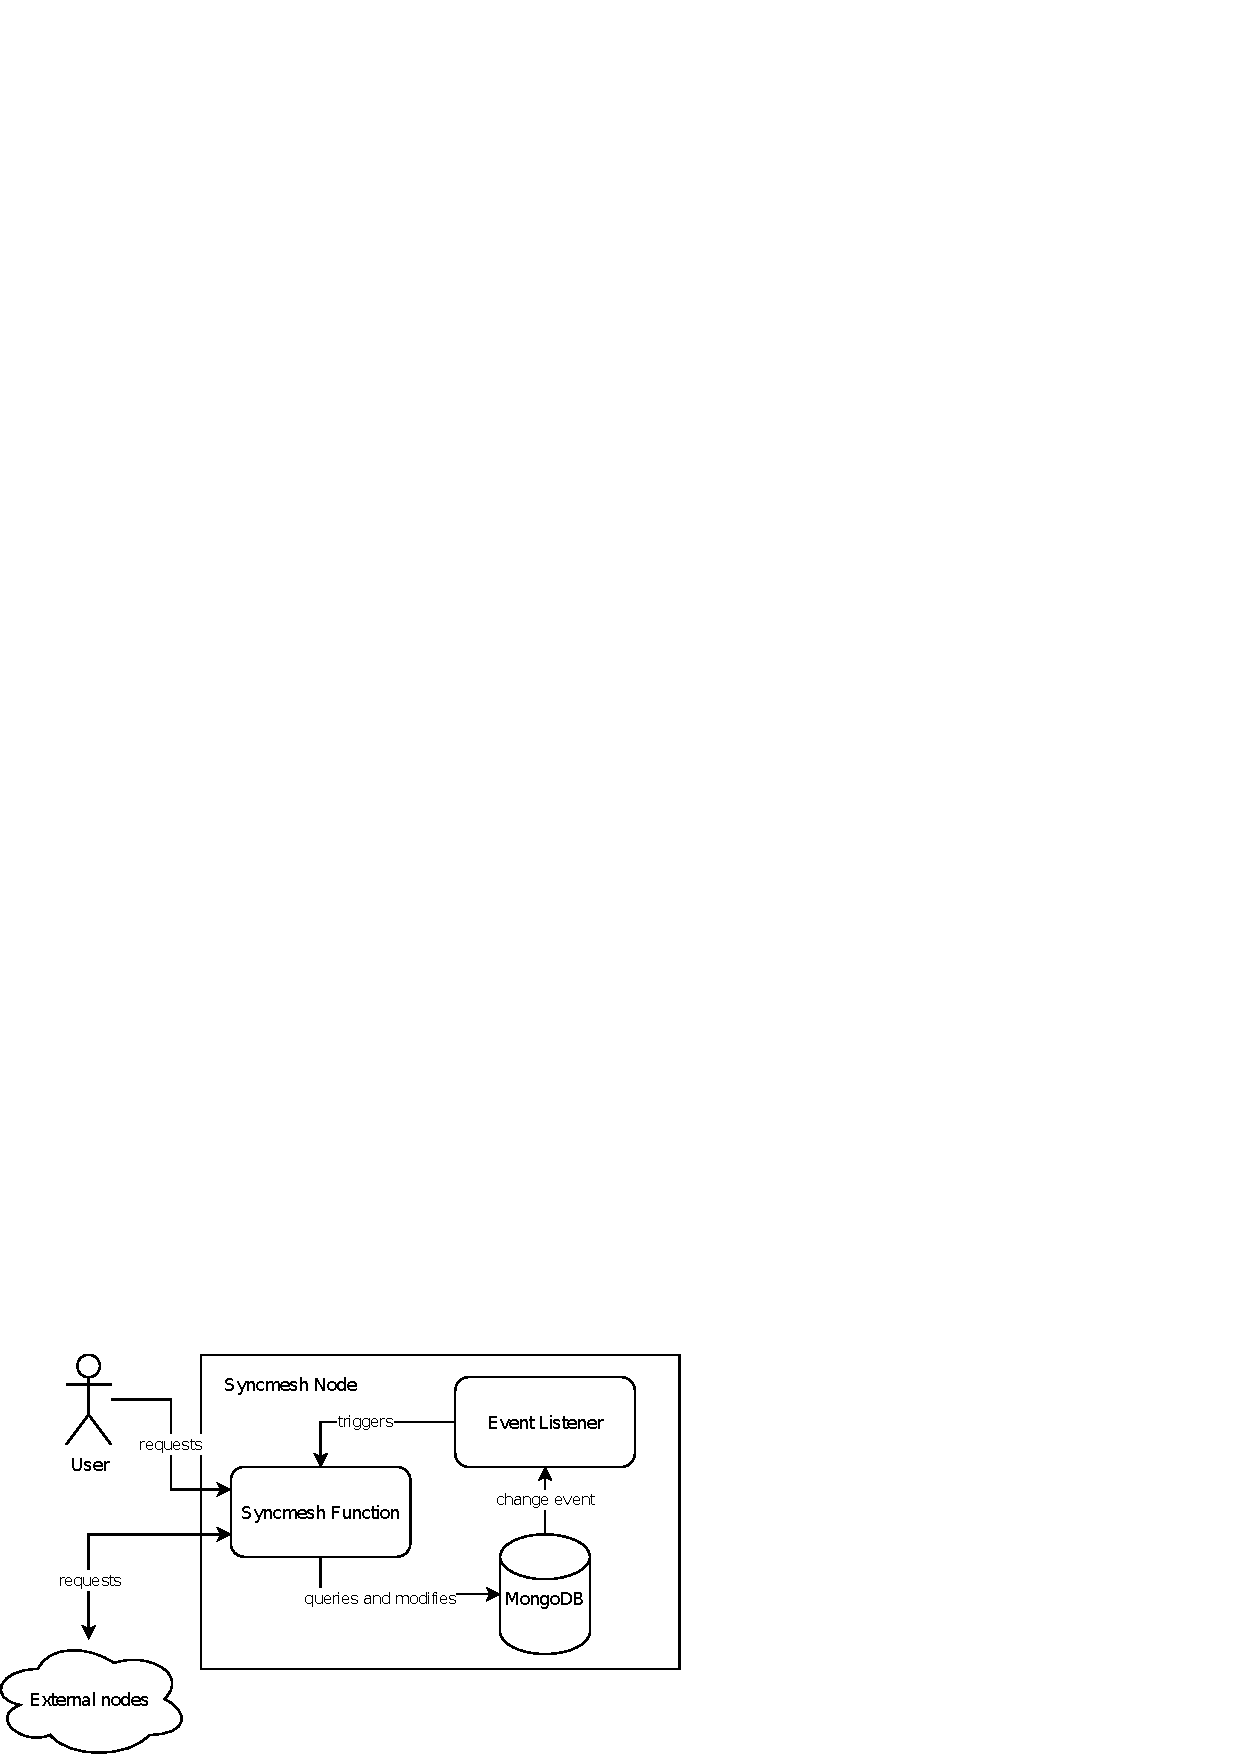
\includegraphics[width=\linewidth]{img/syncmesh_node.pdf}
	\caption{Architecture of a Syncmesh Node}
    \label{fig:syncmesh-node} % don't forget, label always at the end!
\end{figure}

To enable this, the architecture of a so-called "Syncmesh Node", depicted in \Cref{fig:syncmesh-node}, contains several key components:

\begin{itemize}
    \item A deployed "Syncmesh function" which parses and handles user and external node requests
    \item A corresponding local database which the function can access, both with read and write operations
    \item A separately instantiated database listener, which forwards new change events in the database to the Syncmesh function
\end{itemize}

One of the core components of each node is the aforementioned Syncmesh function. It is the core and main handler of any given request inside the distributed mesh of Syncmesh Nodes, acting as the node interface. All data and meta operations, such as collection, aggregation or saving and modification of stored external nodes are handled by the function. Additionally, the Syncmesh function forwards events registered by the database listener to subscribed nodes, thus enabling decentralized data replication and event-driven mechanisms. The specific implementation of the function and its mechanisms will be discussed in \Cref{Chap:Prototype}. It is important to note that the function itself is stateless, conforming to the \ac{faas} design principles and enabling horizontal scalability.

The attached database has no internal logic apart from read/write operations provided out-of-the-box, aggregation queries and the ability to register change listeners. The latter becomes relevant for our database listener component. The listener is responsible for registering modifications of database entries and forwarding them to the Syncmesh function, which in turn distributes the database change to subscribed external functions, after modifying the database change into the appropriate request format.

\section{Prototype}\label{Chap:Prototype}
To address the architecture conceptualized in \Cref{Sec:Architecture}, this chapter deals with the specific coordination, function lifecycle and query or data manipulation mechanisms of our proposed solution. Additionally, a description of the database structure as well as the node deployment process is described.

\subsection{Used Technologies}\label{Sec: Techstack}
The foundation and underlying framework for Syncmesh is the open-source framework OpenFaaS, which contains function deployment, management and event handling. Also described in \Cref{Sec:Architecture} and depicted in \Cref{fig:syncmesh-node}, each node of the mesh has an own local database deployment. For our solution, we opted for MongoDB after an initial research phase, as it provides benefits of event listeners and a schema-less structure out-of-the-box, in addition to internal data aggregation mechanisms. As the nodes communicate in a manner of sending and receiving HTTP requests, a defined protocol was imperative. For standardizing this communication between functions, \ac{rest} enables each node to send and receive specified requests by defined constraints. To further simplify the goal of coordinating data requests, GraphQL was chosen as a query language. This enables a compression of extensive queries into a single query string that can be passed as a parameter of the \ac{rest} request.

For deployment and evaluation, faasd\footnote{https://github.com/openfaas/faasd}, a modified, tinier version of OpenFaaS was of relevance. The requirements described in \Cref{Sec:Architecture} and given the nature of \ac{iot} devices themselves, the deployment was constrained to a single host with low system requirements, which faasd fulfills. Additionally Terraform was used to automate deployment and testing workflows as a manual cluster deployment was proven too time-consuming and not consistently reproducible.

\subsection{Node Communication and Lifecycle}\label{sec:node-lifecycle}
The core mechanism behind the data replication and communication capabilities of Syncmesh is the node communication process. The communication happens on the application layer, as functions receive and send HTTP requests to and from each other.

For this, we introduce a unified request schema that applies to all Syncmesh functions. Each request is contained within a single \ac{json} body and has the following properties:

\begin{itemize}
    \item \textit{query} which contains the GraphQL query for fetching or mutating specific data entries in the node database
    \item \textit{database} to address the database the data will be queried from
    \item \textit{collection} for specifying the collection inside the above stated database
    \item \textit{request\_type} to specify whether the collection data that is queried will be just collected or aggregated to averages. If a mutation operation needs to be performed, this parameter is optional
    \item \textit{external\_nodes} as an optional parameter to specify the addresses of external nodes
    \item \textit{use\_meta\_data} which determines whether locally stored external nodes should be used for querying or aggregating data
    \item \textit{radius} as an optional parameter to define a geographic radius in which external nodes are queried
\end{itemize}

To enable data collection from multiple nodes, each Syncmesh node has an own integrated data collection algorithm. After collecting a list of locally stored external nodes as well as the node addresses passed by the user, the node forwards the initial user request to each of the external nodes. After receiving the responses containing the localized data, it is combined into a unified data list, which is then sent as a response to the user who initiated the initial request. Depending on whether aggregation or collection was selected, the final response is either a complete list of all data entries contained in all queried nodes (collection) or the combined average of these entries (aggregation). Mutation operations, such as modifying, deleting, or creating a new entry, are not forwarded.

\begin{figure}[!h]
	\centering
		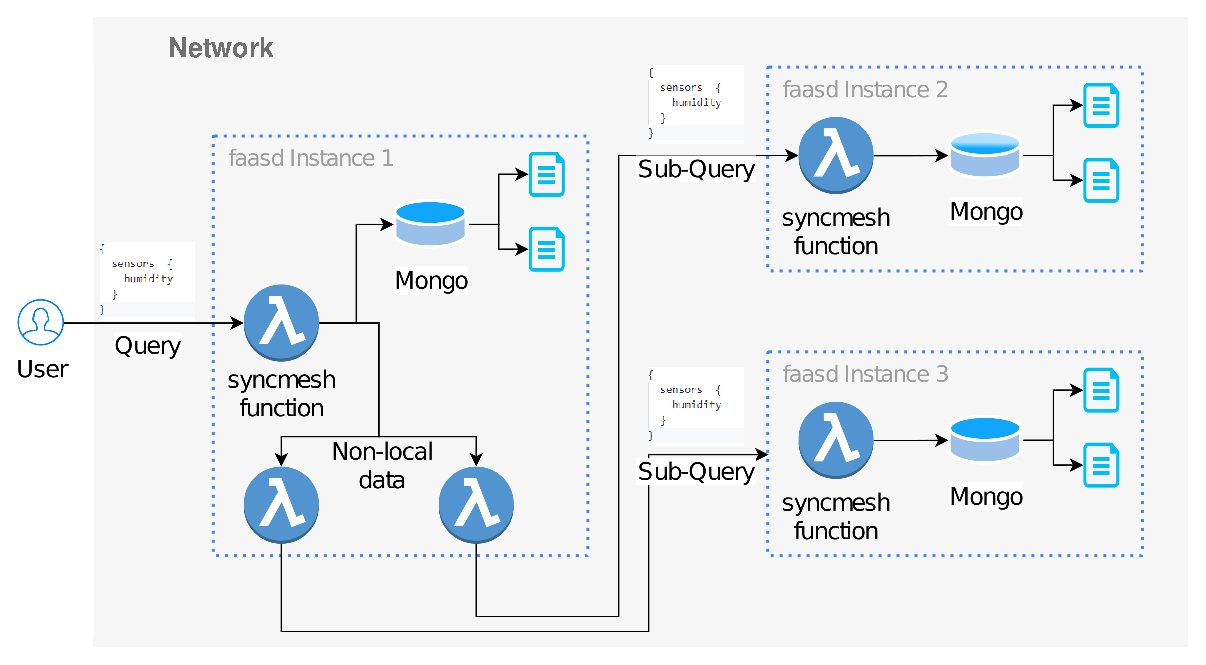
\includegraphics[width=\linewidth]{img/network_request_bigger.eps}
	\caption{Process of a Syncmesh request with forwarding to external nodes}
    \label{fig:syncmesh-request} % don't forget, label always at the end!
\end{figure}

Thus, we establish a function request lifecycle, outlined in the following steps and depicted in \Cref{fig:syncmesh-request}:

\begin{enumerate}
    \item An initial HTTP request containing the aforementioned properties as well as the GraphQL query is made to the function, as seen on the left side of \Cref{fig:syncmesh-request}
    \item The function queries internal data first and collects it into an array or aggregates it into average values for each property
    \item The function sends out the same query to both saved and specified external nodes, waiting for any kind of response with each. The protocol does not repeat in case of an unsuccessful request, if one node returns an error, the iteration continues with the next node
    \item The responses are either combined into the aforementioned array, or aggregated together with the local results
    \item The final result is then returned as a response to the initial request
\end{enumerate}

In addition to the standard lifecycle, an optional preprocessing step is performed if a radius is specified. If this is the case, the Syncmesh function performs a distance calculation using the coordinates of all stored external nodes and the own node. The main assumption is that closer nodes are more relevant to the user, so after a filtering step with the specified radius, the final list is sorted in ascending order by the calculated distance.

\subsection{Meta Requests}\label{sec:meta-requests}
Next to regular data querying and mutation operations, the Syncmesh function also provides an interface to modify locally stored external nodes. This is achieved by using different parameters, which the function recognized and thereby classifies the request as a "meta request". Creation, modification and deletion of nodes is possible, with passed parameters outlined in \Cref{sec:database-structure}. Currently, no mechanisms are provided to automatically assign or discover external nodes, thus the necessity of such a mechanism was evident.

\subsection{Event-driven Requests}\label{sec:event-driven}
As described in \Cref{Sec:Architecture}, each Syncmesh node can contain an event listener that internally triggers the OpenFaaS function. This enables an event-driven architecture, by allowing both subscription to events that occur in an external node, as well as distributing local database events to external nodes. Each stored external node has a \textit{subscribed} flag. If this flag is set to true, any database changes detected by the event listened will be also forwarded to any of the subscribed nodes by the local function. In this case, the response of the subscribed nodes is not considered, so it is a "fire-and-forget"-request.

With the event listener, data replication within subscribed nodes is achieved, by forwarding create, update and delete requests. To determine the relevant document within the other nodes, a so-called "replica ID" is used. The replica ID consists of a concatenation of the address of the initial node and the according internal MongoDB ID of the given document. Thus, a globally unique identifier across all subscribed nodes is persisted and used for external document changes.

\subsection{Database Structure}\label{sec:database-structure}
With MongoDB being used as a local database for a given node, it is important that the distinction of data and metadata is clarified. Data concerns all information recorded by hypothetical weather sensors within the vicinity of the node, while metadata concerns information regarding the node properties, as well as other known external nodes. In the MongoDB instance, this is represented by two databases: \textit{syncmesh} for data collections, and \textit{syncmesh\_meta} for metadata collections. Information about external and the own node is contained within the \textit{nodes} collection within \textit{syncmesh\_meta}. 

For the main data collection, it mirrors the initial dataset with pressure, humidity, temperature, a timestamp, and in some instances, the replica ID as outlined in \nameref{sec:event-driven}.

For metadata, information about a node consists of whether it is its own node, its IP address, location split into both latitude and longitude, what the distance to the own node is and whether the node is subscribed to local database changes. The distance is stored in the document to reduce computational complexity when querying external nodes with the radius parameter. It is recomputed if the location of the node is updated.

\subsection{Node Deployment}
For the deployment of the nodes, we wrote an extensive documentation which can be found on GitHub\footnote{\url{https://github.com/DSPJ2021/syncmesh/wiki}}. In short, the deployment consists of an automated faasd installation with an integration of MongoDB into the faasd container runtime and then a deployment of the Syncmesh function as a normal faasd function. Further workloads e.g. for \nameref{sec:event-driven} or other functions can be deployed via the management command-line interfaces of OpenFaaS and Docker. To make the initial deployment easier and consistent, we packaged the setup into one installation script.


\section{Evaluation}\label{Chap:Eva}

In this chapter we will explain how we benchmarked and compared our solution to other software. We will briefly cover the technical setup, followed by the test results including their subsequent evaluation.

\subsection{Benchmark Definition}\label{Section:Benchmark}
To build a comprehensive benchmark, we followed the principles of \citetitle{Kistowski2015HowBenchmark} \cite{Kistowski2015HowBenchmark}. According to the categorization presented in the work, we conducted a "specification-based" \cite{Kistowski2015HowBenchmark} benchmark - meaning that we only specify input and output parameters which allows for custom implementations of a solution.  

In order to conduct a well-defined benchmark we made sure to adhere to the main criteria for a good benchmark, outlined in the paper: 
\begin{enumerate*}
    \item Relevance
    \item Reproducibility
    \item Fairness
    \item Verifiability and
    \item Usability
\end{enumerate*}.

\subsubsection{Relevance}
The relevance arises through prior research, related work discussed in \Cref{Chap:RelatedWork}, and the inherent necessity of evaluating the performance to see if the proposed solution is feasible.

\subsubsection{Reproducibility}
For a valid comparison, we used the same dataset in each scenario from a real-life \ac{iot} network as described in \Cref{Sec:Architecture}. 
In each scenario the dataset of one sensor was distributed to one node and then replayed as measurements similar to a real sensor.
All software versions and hardware requirements are listed in \autoref{tbl:specification}.

\subsubsection{Fairness}\label{subsub:fairness}
We based all of our tests in a virtual environment which was hosted in \ac{gcp}. 
In order to ensure fairness the experiments have been conducted at different times of day and cross checked for differences. All tests have been run in parallel to minimize dependencies on different workloads that may impact \ac{gcp} itself. 
All Applications only include minimal configuration (read as default settings) with no performance tweaks other than TCP Paket Compression (GZIP for Syncmesh and Snappy for MongoDB\footnote{ \url{https://docs.mongodb.com/manual/reference/configuration-options/\#mongodb-setting-net.compression.compressors}}). 
In order to not run into congestions, we closely monitored network traffic and machine load.

\subsubsection{Verifiability and Usability}

By running our Benchmark on a public cloud provider everyone can verify our results. We provide the Terraform Scripts and additional tooling, e.g. automation via GitHub Actions for each Benchmark. 
Relevant configurations can be directly controlled via Terraform variables. Thus making it easier to reproduce and harder to make any mistakes when changing parameters for the benchmark. 



\subsection{Technical Setup}

We used \href{https://cloud.google.com/}{\acl{gcp}} for reasons of convenience as we had university credits for the platform. 
The Hard- and Software we used can be seen in \autoref{tbl:specification} and we will briefly explain why we chose them.
While testing our benchmark we used "f1-micro" instances and initially thought that we could also use them for the benchmark. But as the data from our first tests has been inconsistent, we found that Google states there are "Shared-core VMs offer bursting capabilities that allow instances to use additional physical for short periods of time." \cite{Google2021General-purposeDocumentation} 
That is why non-shared "n1-standard-1"\footnote{\url{https://cloud.google.com/compute/docs/general-purpose-machines\#n1_machines}} were chosen during our published benchmarks and recommended to do so for the aforementioned reason.
We could not use \ac{cos} because it was not compatible with the faasd container operator which is why we chose Ubuntu as the OS. The software versions tested have been chosen by the currently latest version available. 

\begin{table}[!h]
\caption{Hard and Software Specifications}
\centering
\begin{tabular}{|c|c|}
   \hline
   \multicolumn{2}{|c|}{Hardware} \\ \hline
   CPU & 1 @ 2.60GHz \\
   Memory & 3.75 GB \\ \hline
    \multicolumn{2}{|c|}{Software} \\ \hline
    Ubuntu & \href{https://cloud.google.com/compute/docs/images/os-details#ubuntu_lts}{20.04-lts} \\ 
    MongoDB (mongo, monogs, mongod) & 5.0.2 \\
    faasd & 0.14.2 \\ \hline
\end{tabular}
\label{tbl:specification}
\end{table}

During the benchmarking process, we also made some custom decisions that are stated next. 
For the tests, we used the legacy mongo cli instead of mongosh because the newer version does not support specifying network Compression Parameters\footnote{ \url{https://docs.mongodb.com/manual/reference/program/mongo/\#std-option-mongo.--networkMessageCompressors}}.
For Measuring network traffic we initially wanted to use VPC Flow logs\footnote{\url{https://cloud.google.com/vpc/docs/flow-logs}} which samples the network traffic without impacting the performance. But during testing we noticed some variations in between measurements which has to do with the method VPC Flow logs utilizes. Google does not disclose how they choose the packets that get sampled but write "at most about 10\% of packets at the VM level are processed" \cite{VPCCloud}, which explains the fluctuations. Our next idea was to use Network Mirroring but \ac{gcp} states that Package mirroring is done on the VM that is mirrored. As this influences the performance of the machine either way, we resorted to tcpdump.  
In order to record machine workload, we simply used the native implementation by \ac{gcp} Metrics.

\subsection{Benchmark}

With the goal of having a meaningful comparison to our solution, we implemented three systems: 

\begin{enumerate}
  \item Baseline \newline
  A simple implementation of a sensor network sending the data to a central MongoDB Instance and a Client querying it from there.
  \item Advanced \newline
  A more advanced baseline implementation leveraging sharding to keep original data on a shard on each node. 
  \item Syncmesh \newline
  Our solution as described in \Cref{Chap:Prototype}. 
\end{enumerate}
More detailed information is available in our Wiki. 
To test the systems under different conditions we specified the following parameters:
\begin{itemize}
    \item Number of nodes (3, 6, 9, 12)
    \item Latency (same location, different locations)
    \item Workload (aggregate, collect)
    \item Data Timespan (1, 7, 14, 30 days)
    \item Request count (20, 40, 80)\label{param:request_count}
\end{itemize}
Finally, in order to compare the systems, we recorded the following metrics: 
\begin{itemize}
    \item Network Traffic
    \item \acf{rtt} per Request
    \item Memory and CPU Usage
\end{itemize}
and generated the subsequent results, depicted in \Cref{tbl:benchmark-results-3}:

For different Request Counts, Timespans and Latency Constraints the Systems Metrics all in a linear manner or stay even. In the end, these metrics mostly contributed to check the correct implementation.
Scaling the number of nodes also did not impact any of the systems significantly, at least up to the number of 12 nodes we tested with (see \autoref{tbl:benchmark-results-3} and \autoref{tbl:benchmark-results-6} for a comparison). 
All of the aforementioned will not be covered in more detail in this paper, they are however available in the project repository.

\begin{figure}[!h]
	\centering
		\includegraphics[width=0.7\linewidth]{img/network_advanced.png}
	\caption{The network diagram and traffic for the advanced system.}
    \label{fig:network-advanced}
\end{figure}

The systems differ when inspecting various workloads, as can be seen in \autoref{tbl:benchmark-results-3}. The percentage is given as the deviation from the baseline system. The \ac{rtt} for the Syncmesh and advanced system are both higher, mainly because of the additional requests being made in the background which query the data from the corresponding node instead of a central instance.
Traffic-wise, the advanced scenario deviated from the expected outcome, due to the additional traffic that is needed for internal communication of the MongoDB shards (as can be seen in \autoref{fig:network-advanced}). Our solution performs better for both workloads. 
The "collect" workload might benefit from a better compression ratio (see \Cref{subsub:fairness}) but mainly from the absence of a central instance the data would need to pass through in the baseline system. 
For the "aggregate" workload, Syncmesh is almost 70 times more efficient in its bandwidth usage due to the local aggregation process and general lifecycle, as specified in \Cref{sec:node-lifecycle}.

% For editing the table: https://www.tablesgenerator.com/latex_tables
\begin{table}[]
\caption{Scenario benchmark results for 3 Nodes}
\centering
\begin{tabular}{|l|l|l|l|l|}
\hline
           & \multicolumn{2}{l|}{Traffic (in MB)}                                                                                      & \multicolumn{2}{l|}{RTT (in ms)}                                                                                  \\ \hline
system & aggregate                                                    & collect                                                    & aggregate                                               & collect                                                 \\ \hline
baseline   & \begin{tabular}[c]{@{}l@{}}34.74\\ (+0.0\%)\end{tabular}     & \begin{tabular}[c]{@{}l@{}}72.69\\ (+0.0\%)\end{tabular}   & \begin{tabular}[c]{@{}l@{}}75\\ (+0.0\%)\end{tabular}   & \begin{tabular}[c]{@{}l@{}}76\\ (+0.0\%)\end{tabular}   \\ \hline
advanced   & \begin{tabular}[c]{@{}l@{}}36.95\\ (+6.0\%)\end{tabular}     & \begin{tabular}[c]{@{}l@{}}275.05\\ (+73.6\%)\end{tabular} & \begin{tabular}[c]{@{}l@{}}118\\ (+36.1\%)\end{tabular} & \begin{tabular}[c]{@{}l@{}}114\\ (+33.2\%)\end{tabular} \\ \hline
syncmesh   & \begin{tabular}[c]{@{}l@{}}0.56\\ (-6134.3\%)\end{tabular} & \begin{tabular}[c]{@{}l@{}}62.39\\ (-16.5\%)\end{tabular}  & \begin{tabular}[c]{@{}l@{}}110\\ (+31.2\%)\end{tabular} & \begin{tabular}[c]{@{}l@{}}110\\ (+30.7\%)\end{tabular} \\ \hline
\end{tabular}
\label{tbl:benchmark-results-3}
\end{table}


\begin{table}[]
\caption{Scenario benchmark results for 6 Nodes}
\centering
\begin{tabular}{|l|l|l|l|l|}
\hline
           & \multicolumn{2}{l|}{Traffic (in MB)}                                                                                     & \multicolumn{2}{l|}{RTT (in ms)}                                                                                  \\ \hline
system & aggregate                                                  & collect                                                     & aggregate                                               & collect                                                 \\ \hline
baseline   & \begin{tabular}[c]{@{}l@{}}66.10\\ (+0.0\%)\end{tabular}   & \begin{tabular}[c]{@{}l@{}}288.15\\ (+0.0\%)\end{tabular}   & \begin{tabular}[c]{@{}l@{}}129\\ (+0.0\%)\end{tabular}  & \begin{tabular}[c]{@{}l@{}}130\\ (+0.0\%)\end{tabular}  \\ \hline
advanced   & \begin{tabular}[c]{@{}l@{}}45.88\\ (-44.1\%)\end{tabular}  & \begin{tabular}[c]{@{}l@{}}508.17\\ (+43.3\%)\end{tabular}  & \begin{tabular}[c]{@{}l@{}}190\\ (+32.4\%)\end{tabular} & \begin{tabular}[c]{@{}l@{}}183\\ (+28.7\%)\end{tabular} \\ \hline
syncmesh   & \begin{tabular}[c]{@{}l@{}}1.02\\ (-6370.5\%)\end{tabular} & \begin{tabular}[c]{@{}l@{}}107.57\\ (-167.9\%)\end{tabular} & \begin{tabular}[c]{@{}l@{}}161\\ (+20.3\%)\end{tabular} & \begin{tabular}[c]{@{}l@{}}162\\ (+19.6\%)\end{tabular} \\ \hline
\end{tabular}

\label{tbl:benchmark-results-6}
\end{table}


\begin{figure}[!h]
	\centering
	    \includegraphics[width=0.7\linewidth]{img/network_baseline-aggregate.png}
	\caption{The network diagram and traffic for the baseline system with the workload "aggregate".}
    \label{fig:network-baseline}
\end{figure}

The stark contrast is especially visible when comparing the Baseline (\autoref{fig:network-baseline}) to the Syncmesh (\autoref{fig:network-syncmesh}) traffic diagram, which shows the full ingest to the central server for baseline and only the result of the aggregated values for the Syncmesh system.

\begin{figure}[!h]
	\centering
		\includegraphics[width=0.7\linewidth]{img/network_syncmesh-aggregate.png}
	\caption{The network diagram and traffic for the Syncmesh system with the workload "aggregate".}
    \label{fig:network-syncmesh}
\end{figure}

The Memory and CPU Usage of all systems is relatively low. 
However, the Syncmesh system uses significantly more memory, which might be explained by the dockerized installation. 

But overall, all systems consume little memory (see \autoref{fig:memory}).

\begin{figure}[!h]
	\centering
		\includegraphics[width=0.7\linewidth]{img/ram_comparison_aggregated_9.png}
	\caption{Memory Usage Comparison\\ Calculated by comparing the used Memory over time with the overall Memory Capacity.}
    \label{fig:memory}
\end{figure}

On the other hand, Syncmesh uses moderately more CPU for the "collect" workload than other systems, but less CPU for the "aggregate" workload, mainly because it might not need to move as much data as the other systems (see \autoref{fig:cpu}). 

\begin{figure}[!h]
	\centering
		\includegraphics[width=0.7\linewidth]{img/cpu_comparison_aggregated_9.png}
	\caption{CPU Usage Comparison\\
	Calculated by the mean of CPU Usage over time scaled by the number of instances: \\ 
	$ Usage = mean(CPU Measurements) * Number Of Machines$.}
    \label{fig:cpu}
\end{figure}

Overall, our proposed system performs well. It adds latency, but performs better for both the aggregate and collect scenarios, traffic-wise. It uses significantly more memory due to the involved Virtualization Technologies and uses less or more CPU based on the workload. 

\newpage
\section{Conclusion}\label{Chap:Conclusion}

With this paper, we proposed and evaluated Syncmesh, a distributed data management system using \ac{faas} as its main propagation and coordination tool. This was achieved by implementing a custom function that handles data requests in a unified manner, thus enabling users to manage and query data in a distributed and scalable environment. In combination with a local database and an event listener, Syncmesh can be used to communicate with other instances that use a similar configuration or other (Syncmesh) functions. 

Our evaluation concluded that the Syncmesh infrastructure performs on a sufficient level in comparison to traditional, centralized solutions. A marginal RTT increase does exist, however, contrasting a reduction in traffic for both collection and aggregation workloads for a reasonable CPU and RAM usage increase.


\subsection{Outlook}\label{Sec:Outlook}
After an initial benchmarking and evaluation phase, we determined that the proposed solution performs adequately to an acceptable extent. However, further work is needed with regard to the evaluation, extending scenarios, and performing a stress analysis for more rare-case scenarios. Adding other systems that closely resemble the Syncmesh functionality would also greatly benefit the relevance of the benchmark.

In addition to the evaluation, the Syncmesh function itself can be further generalized to support data management of any document kind, as it is currently adapted towards the evaluated dataset. Furthermore, several steps can be taken to optimize the query distribution and replication mechanism, such as the possibility of data offloading if a specific node has storage limitations. Finally, when considering the general direction of the research regarding our proposal, the focus can be extended towards mechanisms of a centralized broker for node coordination and discovery, as currently, the latter is performed in a manual manner.

\printbibliography

%\newpage
%\onecolumn
%\appendix

%\subsection{Project Guide}\label{appendix:docu}


%\begin{figure}[!h]
%	\centering
		%\includegraphics[width=\textwidth, height=0.9\textheight, keepaspectratio=true]{img/documentation.png}
%	\caption{Caption}
%\end{figure}

%\FloatBarrier


%\FloatBarrier

%\vspace{12pt}
\end{document}
